%% LyX 1.5.5 created this file.  For more info, see http://www.lyx.org/.
%% Do not edit unless you really know what you are doing.
\documentclass[a4paper,czech,czech,openright,cleardoubleempty,BCOR10mm,DIV11]{scrreprt}
\usepackage[T1]{fontenc}
\usepackage[utf8]{inputenc}
\usepackage{array}
\usepackage{longtable}
\usepackage{varioref}
\usepackage{wrapfig}
\usepackage{fancybox}
\usepackage{calc}
\usepackage{framed}
\usepackage{url}
\usepackage{graphicx}
\usepackage{color}
\usepackage{float}
\usepackage{svg}
\usepackage{amsmath}
\usepackage{makecell}
\usepackage{fourier} 
\usepackage{pdfpages}

\makeatletter

%%%%%%%%%%%%%%%%%%%%%%%%%%%%%% LyX specific LaTeX coěmmands.
\providecommand{\LyX}{L\kern-.1667em\lower.25em\hbox{Y}\kern-.125emX\@}
\newcommand{\lyxline}[1][1pt]{%
  \par\noindent%
  \rule[.5ex]{\linewidth}{#1}\par}
\newcommand{\noun}[1]{\textsc{#1}}
%% Special footnote code from the package 'stblftnt.sty'
%% Author: Robin Fairbairns -- Last revised Dec 13 1996
\let\SF@@footnote\footnote
\def\footnote{\ifx\protect\@typeset@protect
    \expandafter\SF@@footnote
  \else
    \expandafter\SF@gobble@opt
  \fi
}

\expandafter\def\csname SF@gobble@opt \endcsname{\@ifnextchar[%]
  \SF@gobble@twobracket
  \@gobble
}
\edef\SF@gobble@opt{\noexpand\protect
  \expandafter\noexpand\csname SF@gobble@opt \endcsname}
\def\SF@gobble@twobracket[#1]#2{}
%% Because html converters don't know tabularnewline
\providecommand{\tabularnewline}{\\}

%%%%%%%%%%%%%%%%%%%%%%%%%%%%%% Textclass specific LaTeX commands.
\newenvironment{lyxcode}
{\begin{list}{}{
\setlength{\rightmargin}{\leftmargin}
\setlength{\listparindent}{0pt}% needed for AMS classes
\raggedright
\setlength{\itemsep}{0pt}
\setlength{\parsep}{0pt}
\normalfont\ttfamily}%
 \item[]}
{\end{list}}

%%%%%%%%%%%%%%%%%%%%%%%%%%%%%% User specified LaTeX commands.
%<-------------------------------společná nastavení------------------------------>
\usepackage[czech]{babel}%počeštění názvů (Obsah, Kapitola, Literatura atp.)
\usepackage[]{hyperref} %odkazy v  pdf jsou klikací s barevnými rámečky
\usepackage[numbers,sort&compress]{natbib} %balíček pro citace literatury  
\usepackage{hypernat}%interakce mezi hyperref a natbib
\newcommand{\BibTeX}{{\sc Bib}\TeX}%BibTeX logo
\hypersetup{   % Nastavení polí PDF dokumentu 
pdftitle={Evaluation of Container-based Virtualization for standard company environment},%   
pdfauthor={Pavel Cizinsky},%  
pdfsubject={},%   
pdfkeywords={Docker, Kubernetes, Kotejner, Virtualizace}%                             
}
\usepackage{multicol}




%<-----------------------------volání stylů----------------------------------------->
% (znak % je označení komentáře: co je za ním, není aktivní)
%<------------------------------------písmo----------------------------------------->
%\usepackage{packages/bc-latinmodern}
%\usepackage{packages/bc-times}
\usepackage{packages/bc-palatino}
%\usepackage{packages/bc-iwona}
%\usepackage{packages/bc-helvetika}


%<------------------------------záhlaví stránek------------------------------------>
%\usepackage{packages/bc-headings}
\usepackage{packages/bc-fancyhdr}

%<------------------------------hlavičky kapitol------------------------------------>
%\usepackage{packages/bc-neueskapitel}
%\usepackage{packages/bc-fancychap}

\makeatother

\usepackage{babel}

%java code block%

\usepackage{listings}
\usepackage{color}

\definecolor{dkgreen}{rgb}{0,0.6,0}
\definecolor{gray}{rgb}{0.5,0.5,0.5}
\definecolor{mauve}{rgb}{0.58,0,0.82}

% syntax highlight pro jazyk Javascript %
\definecolor{purple}{rgb}{0.65, 0.12, 0.82}
\lstdefinelanguage{JavaScript}{
  keywords={break, case, catch, const, continue, debugger, default, delete, do, else, false, finally, for, function, if, in, instanceof, let, new, null, return, switch, static, this, throw, true, try, typeof, var, void, while, with},
  morecomment=[l]{//},
  morecomment=[s]{/*}{*/},
  morestring=[b]',
  morestring=[b]",
  ndkeywords={class, constructor, export, extends, boolean, throw, implements, import},
  keywordstyle=\color{blue}\bfseries,
  ndkeywordstyle=\color{gray}\bfseries,
  identifierstyle=\color{black},
  commentstyle=\color{purple}\ttfamily,
  stringstyle=\color{red}\ttfamily,
  sensitive=true
}

\lstset{,
  language=Javascript,
  aboveskip=3mm,
  belowskip=3mm,
  showstringspaces=false,
  columns=flexible,
  inputencoding=utf8,
    extendedchars=true,
    literate=%
    {á}{{\'a}}1
    {č}{{\v{c}}}1
    {ď}{{\v{d}}}1
    {é}{{\'e}}1
    {ě}{{\v{e}}}1
    {í}{{\'i}}1
    {ň}{{\v{n}}}1
    {ó}{{\'o}}1
    {ř}{{\v{r}}}1
    {š}{{\v{s}}}1
    {ť}{{\v{t}}}1
    {ú}{{\'u}}1
    {ů}{{\r{u}}}1
    {ý}{{\'y}}1
    {ž}{{\v{z}}}1
    {Á}{{\'A}}1
    {Č}{{\v{C}}}1
    {Ď}{{\v{D}}}1
    {É}{{\'E}}1
    {Ě}{{\v{E}}}1
    {Í}{{\'I}}1
    {Ň}{{\v{N}}}1
    {Ó}{{\'O}}1
    {Ř}{{\v{R}}}1
    {Š}{{\v{S}}}1
    {Ť}{{\v{T}}}1
    {Ú}{{\'U}}1
    {Ů}{{\r{U}}}1
    {Ý}{{\'Y}}1
    {Ž}{{\v{Z}}}1,
  basicstyle={\small\ttfamily},
  xleftmargin=1cm,
  keywordstyle=\color{blue},
  commentstyle=\color{dkgreen},
  stringstyle=\color{mauve},
  breaklines=true,
  breakatwhitespace=true,
  tabsize=3
}
\usepackage{url}
\makeatletter
\g@addto@macro{\UrlBreaks}{\UrlOrds}
\makeatother

% vlastni package
\usepackage{placeins}
\usepackage{multirow}
\usepackage{pdfpages}
% fonty popisku
\usepackage[font=small,labelfont=bf]{caption}
% radkovani 
\renewcommand{\baselinestretch}{1.2}
\renewcommand*{\lstlistingname}{Kód} %prejmenovani lstlisting
\renewcommand*{\lstlistlistingname}{Seznam ukázek kódu}
% vlastni styly tabulek
\newcolumntype{C}[1]{>{\centering\arraybackslash}m{#1}}
\begin{document}

\cleardoublepage{}~\thispagestyle{empty}\begin{center}\pagenumbering{roman}\vspace{10mm}


\textsf{\textsc{\noun{\LARGE Univerzita Hradec Králové}}}\\
\vspace{0.5em}
\textsc{\noun{\LARGE Fakulta informatiky a managementu}}\\
\vspace*{1em}
\textsf{\textsc{\noun{\Large katedra informačních technologií }}}


%%% Aby vložení loga  správně fungovalo, je třeba mít soubor uhk.png nahraný v adresáři logo,
%%% tj. v adresáři, kde se nachází překládaný zdrojový soubor. 
\vspace{4cm}

\textsf{\huge BAKALÁŘSKÁ PRÁCE}{\huge \par}

\vspace{15mm}


\textsf{\LARGE Diplomova prace}{\LARGE \par}

\vspace{10mm}


\end{center} 

\vspace*{\fill}


\vspace{10mm}


\begin{description}
%studijni obor???
\item [{{\large Autor:}}] \noindent \textsf{\large Jan Cach}{\large \par}
\item [{{\large Studijní obor:}}] \noindent \textsf{\large Aplikovaná informatika}{\large \par}
\item [{{\large Vedoucí~práce:}}] \noindent \textsf{\large Ing. Jakub Pavlík, MSc.}{\large \hfill{}}\textsf{\large Hradec Králové, 2019}{\large{}
% doplňte rok vzniku vaší bakalářské práce
}{\large \par}
\end{description}

\clearpage{}
~\thispagestyle{empty}{\small ~\vfill{}
}{\small \par}

\noindent {\small \vfill{}
 % nastavuje dynamické umístění následujícího textu do spodní části stránky
~}{\small \par}

\noindent {\small Prohlašuji, že jsem bakalářskou práci vypracoval samostatně a uvedl jsem všechny použité prameny a literaturu.}{\small \par}

{\small \bigskip{}
}\noindent {\small{} V Horním Jelení dne \today\hspace{\fill}Jan Cach}\\
{\small{} % doplňte patřičné datum, jméno a příjmení
}{\small \par}

{\small %%%   Výtisk pak na tomto míste nezapomeňte PODEPSAT!
%%%                                         *********
}{\small \par}

\clearpage{}
~\thispagestyle{empty}{\small ~\vfill{}
}{\small \par}

\noindent {\small Rád bych poděkoval Ing. Jakubu Pavlíkovi, MSc. za odborné vedení práce, podnětné rady a čas, který mi věnoval. \newpage{}}{\small \par}
\clearpage{}
~\thispagestyle{empty}{\small ~\vfill{}
}{\small \par}
\noindent {\small \vfill{}
 % nastavuje dynamické umístění následujícího textu do spodní části stránky
~}{\small \par}
\section*{Anotace}
Tato bakalářská práce pojednává o kontejnerové virtualizaci, zabývá se problematikou nasazení kontejnerů do standardního firemního prostředí. První část je věnována představení virtualizace obecně a její porovnání s kontejnerovou virtualizací. Následně je řešena problematika orchestrace a ovládání kontejnerového prostředí. Čtvrtá a pátá kapitola je věnována analýze a převodu aplikace do kontejnerů, součástí  kapitoly pět je praktická ukázka funkčnosti orchestrátoru. Cílem této práce je seznámení čtenáře s konceptem kontejnerů a zjistit jejich využitelnost v produkčním prostředí a možnost převodu klasické aplikace do kontejnerů.
\subsubsection*{Klíčová slova}
Docker, Kubernetes, Cluster, Kontejnery, Virtualizace

\section*{Annotation}
Title: Evaluation of Container-based Virtualization for standard company environment
\vspace{0.5cm}\FloatBarrier
This Bachelor’s thesis describes container-based virtualization especially the issues in its use in standard company environment. The first part is dedicated to intruducing general virtualization and its comparison to container-based virtualization. Afterward is tackled the troubleshooting of orchestration and control of the container-based environment.
The fourth and fifth chapters are devoted to the analysis and conversion of application into containers. Practical example of the orchestration's functionality is included in chapter five.
The aim of this work is to familiarize the reader with the concept of containers and to find out their applicability in the production environment as well as the ability to convert a classic application into containers.

\subsubsection*{Key words}
Docker, Kubernetes, Cluster, Containers, Virtualization

\noindent {\small ~\vfill{}
}{\small \par}

\cleardoublepage{}\thispagestyle{empty}{\small \tableofcontents{}% vkládá automaticky generovaný obsah dokumentu
\cleardoublepage{}}{\small \par}

\chapter{Úvod}
\pagenumbering{arabic}
\setcounter{page}{1}
\section{Směr Cloud Computingu}
Označení Cloud computing je některými odborníky považováno za nové paradigma, někteří dokonce mluví o nové technologii, která umožňuje přístup k výpočetním zdrojům a službám přes internet \cite{bohm2010cloud}. Cloud computing, často označovaný pouze jako cloud, tak dovoluje jednotlivcům, malým firmám a dalším subjektům jednoduchý přístup k výpočetnímu výkonu z pohodlí domova či kanceláře za přijatelnou cenu, bez nutnosti spravovat celou výpočetní infrastrukturu. Uživatelé jsou tak odstíněni od konfigurace serverů a síťových zařízení a služeb samotných. \newline
Podle \cite{cc2011principles} lze na Cloud computing nahlížet jako na využívání elektřiny. Elektřinu využíváme jako službu. Nezajímáme se o to jak se elektřina vyrábí a jak je dodávána do jednotlivých elektrických zásuvek v našem pokoji. My pouze připojíme zařízení do elektrické zásuvky a očekáváme, že například nabije náš telefon či počítač. Pokud tento příklad přeneseme do oblasti IT, znamená to, že uživatelé jsou odstínění od vnitřního fungování nějaké služby nebo použitých technologiích. Jako příklad může být brána služba cloudového uložiště fotografií. Pro uživatele je důležité, že si může fotografie prohlížet  z různých zařízení přes internet odkudkoliv a kdykoliv. Ostatní problémy jako jsou uložení a záloha těchto dat, webové rozhraní pro práci s fotografiemi a další je ponecháno na poskytovateli služby. \newline
Některé instituce, akademičtí pracovníci či IT inženýři vytvořili definice a charakteristiky  popisující Cloud computing. Například Americký národní institut standardů a technologií (NIST) \cite{mel2011nist}, definuje cloud computing následovně:
Cloud computing je model pro pohodlný síťový přístup ke skupině konfigurovatelných výpočetních zdrojů, jako jsou počítačové sítě, servery, datová uložiště, aplikace a služby, které jsou dostupné odkudkoliv a okamžitě na vyžádání. Tyto zdroje mohou být rychle vytvořeny a uvolněny  s vyvinutím minimálního úsilí nebo minimální interakce od provozovatele dané služby. \newline 
Definice ze zdroje \cite{Vaquero-cloud-definition} zmiňuje, že uživatelé platí pouze za zdroje, které skutečně využívají podle sjednaných podmínek. Tento postup se nazývá pay-per-use model. Znamená to žádné pevně stanovené poplatky bez ohledu na to zda zákazník využívá polovinu přidělených zdrojů nebo se využití zdrojů blíží 100 \%. Díky tomu je možné si například vypočítat náklady na provozování služby u různých firem a rozhodnout se tak pro nejvhodnější platformu. \newline
    Armbrust a jeho kolegové z Kalifornské Univerzity v Berkeley \cite{Ambrust2009}, shrnují cloud computing do 3 bodů. Prvním bodem je zdání, že uživatel má k dispozici nekonečný objem výpočetních zdrojů. Z tohoto důvodu není potřeba dopředu plánovat zda bude k dispozici dostatek zdrojů, zdroje jsou dynamicky přidávány a odebírány na požádání. Druhým bodem je skutečnost, že není potřebné uzavírat žádné předběžné závazky ze strany uživatele. Toto dovoluje firmám začít s malým počtem zdrojů a postupně navyšovat zdroje s rostoucími potřebami. Třetím a posledním bodem je zde platit za využívané zdroje ve velice krátkém horizontu, např. hodin nebo dní a poté je uvolnit podle potřeb.

\section{Servisní modely cloud computingu}
Cloud computing můžeme rozdělit do tří kategorií podle služeb, která má daný model poskytovat. Zmíněnými modely jsou Infrasracture as a service (IaaS), Platform as a service (PaaS) a Software as a service (SaaS). Jednotlivé modely se liší ve využítí a účelu pro jaký si je společnost pořizuje. V následujích odstavcích jsou jednotlivé modely blíže představeny. 

\subsection{Infrastructure as a Service}
Z obrázku \cite{cloud-computing-service-model} vyplývá, že IaaS je základem cloudu a nachází se v nejnižší vrstvě celého cloud stacku. Zákazník dostává k dispozici infrastruktu a vše co se nachází nad infrastrukturou jako jsou data, databáze, aplikace a prostředí pro běh aplikací si zákazník ovládá a spravuje sám. Poskytovatel infrastruktury je zodpovědný za fyzické servery, networking, storage a virtualizační vrstvu zajištující vytváření, mazání a správu virtuálních serverů pro lepší využití zdrojů. To znamená, že poskytovatel spravuje fyzické servery včetně disků, pamětí a zdrojů. Dále obstarává konektivitu mezi servery, spravuje switche a routery. Poskytovatel také monitoruje infrastrukturu aby mohl vhodně a včas reagovat na nastalé problémy.\newline
Dostupnost těchto služeb nebo čas do kterého musí poskytovatel adekvátně zareagovat je definována pomocí SLA smlouvy, která je sjednána mezi poskytovatelem služby a zákazníkem \cite{Rongdong}.
Jednotlivé zdroje jako jsou servery, uložiště atd. jsou většinou rozděleny do  menších skupin které jsou poté přiděleny různým uživatelům podle jejich potřeb. Takovými uživateli mohou být například různé firmy nebo rozdílné vývojové týmy v rámci jedné společnosti. Tento způsob vede k lepší správě a využití zdrojů. Uživatelé mají přehled o aktuálním vytížení, kapacitě jednotlivých zdrojů, díky čemuž mohou plánovat případné navýšení kapacity uložiště nebo RAM.\newline
    Výhodou pro uživatele je, že nemusí vlastnit datacentrum se servery, chlazením, monitoringem a dalšími technologiemi, které jsou velice nákladné na pořízení a správu. Nemusí také řešit nákup hardwaru, výměnu starých nebo vadných kusů atd. Zákazníci využívající IaaS nemusí mít odborníky na  problematiku infrastruktury. Všechny tyto aspekty šetří pořizovací i provozní náklady. Při modelu pay-per-use firmy platí pouze za zdroje které využívají a pouze po dobu jakou je využívají. Další výhodou je flexibilita. Uživatelé mají možnost dynamicky přidávat a odebírat zdroje a pružně tak reagovat na velké vytížení, případně šetřit zdroje a peníze při malém vytížení. Zákazníci musí zvážit rizika spojená s bezpečností a důkladně si zjistit podmínky týkající se ztráty nebo odcizení dat, protože data jsou uložena v uložišti, které nejsou ve vlastnictví zákazníka stejně tak tok dat skze sít.\newline
    Mezi společnosti, které nabízejí IaaS patří AWS EC2 (Amazon elastic cloud computing), nebo společnost BlueLock  \cite{salah2011performance}. IaaS řešení poskytuje i Google s nástrojem Google Compute Engine. Dalším významným řešením je open source produkt OpenStack. Jedná se o komunitní projekt a  mnoho společností aktivně přispívá do tohoto projektu. Existuje mnoho společností, které nabízejí svou upravenou verzi OpenStacku \cite{singh2014critical}.

\subsection{Platform as a Service}
    Platform as a service, zkráceně PaaS, je vývojářská platforma podporující plnohodnotný životní cyklus aplikace. PaaS umožňuje uživatelům cloudu vyvíjet cloudové služby a aplikace přímo v prostředí PaaS cloudu \cite{dilon2010cloud}.\newline
         V PaaS modelu poskytování služeb je uživatel zodpovědný pouze za aplikaci a data, se kterými tato aplikace pracuje, proto je používání PaaS pro programátory jednodušší a rychlejší oproti IaaS řešení. Poskytovatel služby má, na rozdíl od IaaS, na starost správu databází, vytváření runtime prostředí pro aplikace nebo provoz webového serveru. Cloud provider poskytuje různé další služby jako jsou verzovací systém nebo lifecycle management aplikace a dále také integrace s různým softwarem třetích stran. Uživatel si nejčastěji vybírá z katalogu jakou databázi bude chtít používat a také runtime prostředí pro programovací jazyk jaký chce uživatel pro vývoj aplikace využít. Výběr jednotlivých zdrojů se liší v závislosti na poskytovateli. Uživatel si jednoduše přes webové rozhraní nebo CLI nástroj vytváří a přidává zdroje které chce využívat. Vše je otázkou několika málo kliknutí. Tento způsob urychluje vývoj aplikace a nenutí programátory učit se konfigurovat různé služby a oni se tak mohou plně věnovat vývoji aplikace.\newline
	      Poskytovatelé služby zjednodušují vývojářům celý proces vývoje aplikace přes správu kódu, nasazení a otestování aplikace, nasazení aplikace do produkce a její další růst, vývoj a monitoring v přehledných grafech a tabulkách. Vývojáři publikují kód do verzovacího systému. Odtud může být pomocí testovacích nástrojů poskytovatelů aplikace nasazena do testovacího provozu a dále po odsouhlasení nasazena do produkce. Poskytovatelé PaaS služeb takto přidávají prvky CI/CD a představují  moderním přístup k tvorbě aplikací.\newline 
	      Další službu, kterou PaaS poskytovatelé nabízí je automatické škálování aplikace. Uživatelé jsou odstíněni od manuálního nastavování loadbalancerů a přidávání dalších webových či databázových serverů. Přidávání serverů pro lepší rozdělení zátěže probíhá automaticky podle předem definovaných pravidel podle toho jak se aplikace rozrůstá. Stejně jako IaaS i PaaS využívá modelu pay-per-use, tedy uživatelé platí pouze za zdroje, které využívají. Jako nevýhodu PaaS řešení může být omezená podpora programovacích jazyků. Každý provozovatel platformy podporuje rozdílné programovací jazyky. Uživatelé jsou tak nuceni vytvořit aplikaci  v jednom z podporovaných jazyků, případně vybrat jiného poskytovatele, který daný jazyk podporuje. Jiný provozovatel může nabízet jiné služby za jiných podmínek. Z tohoto důvodu je nutné dopředu zvážit výběr poskytovatele PaaS služby, protože není snadné a bezbolestné migrovat aplikace mezi různými providery.\newline 
	      Srovnáním PaaS poskytovatelů v práci \cite{lucassen2013ecosystem}, bylo zjištěno že ve sledovaných aspektech si nejlépe vedlo Heroku, následované řešením od společnosti RedHat a dále Azure od firmy Microsoft. Mezi srovávanými služby byly také Google AppEngine, řešení od CloudFoundry a nebo služba poskytovaná firmou dotCloud. Mezi sledovanými aspekty byli například aktivní vývojáři, kteří na dané platformě vyvíjeli za poslední rok nebo počet různých programovacích jazyků provozovaných na dané platformě. Ze závěrů se dá usoudit, že uvedení poskytovatelé PaaS služby pokrývají téměř 100\% trhu.

\subsection{Software as a Service}
Software as a service, zkráceně SaaS, je určen pro koncové uživatele. Poskytovatel Saas spravuje vše od aplikace přes uložení dat až po servery na kterých aplikace běží, tedy celou infrastrukturu i životní cyklus aplikace.  Uživateli stačí se skrze webový prohlížeč, mobilní telefon či jiné zařízení, k aplikaci přihlásit a začít ji používat.
Doručování aplikace jako služby přináší uživatelům nové možnosti jak zrychlit a zkvalitnit práci s nižšími náklady. Pokud si uživatel nějakou službu vybere je otázkou hodiny, než může aplikaci začít používat. Tento proces zahrnuje vytvoření organizace, přidání uživatelů a jejich práv a poté je možné začít aplikaci používat. Tento proces je velmi rychlý oproti klasickému nasazení na servery vlastněné uživatelem. Nevýhodou může být pokud vybraná služba neumožňuje integraci s firemním systémem pro správu uživatelů a jejich práv. Další výhodou oproti desktopové aplikaci je možnost přístupu k aplikaci a jejím datům z různých zařízení a různých lokalit. Většinou stačí uživateli internet pro přístup k aplikaci a není tak vázaný pouze na firemní počítač umístěný v budově firmy.\newline
Velkým plusem SaaS řešení je jasná a dopředu určená cena za využívání dané služby. Poskytovatelé na svých stránkách poskytují kompletní ceník. Uživatel si tak může spočítat a porovnat, které řešení je nejvýhodnější. Změnila se také licenční politika. Například cena služby není vypočítávána podle počtu jader procesoru serveru na kterém je aplikace nasazena, ale podle počtu uživatelů, kteří aplikaci používají. Poskytovatelé dále nabízejí dynamické přidávání a odebírání uživatelů. Přidání zaměstnance do aplikace je opět otázkou minut, stejně jako jeho odebrání. Stejně jako u předchozích typů služeb i zde platí uživatel pouze za to co používá. Šetří tak náklady na IT profesionály a infrastrukturu. Z tohoto důvodu se aplikace stávají více dostupné i malým a středním podnikům, které nemusejí platit infrastrukturu a odborníky, kteří se o ni starají.\newline 
Další významnou složkou pro poskytovatele i uživatele je nasazení nových verzí aplikace a také bezpečnostní aktualizace. Uživatelé běžně dostávají nejnovější verzi aplikace bez nutnosti cokoliv aktualizovat nebo instalovat na svém zařízení. Poskytovatel na druhé straně, může po otestování nové verze aplikace uživatele přesměrovat na novou verzi.\newline 
Společnosti mohou využívat různé druhy aplikací jako jsou aplikace pro řízení vztahů se zákazníkem, kancelářské nástroje, účetní programy a mnoho dalších. První společnost, která nabízela SaaS byla společnost SalesForce, nabízející jejich CRM řešení \cite{salesforce2018}. Dalšími aplikacemi jsou balík nejenom kancelářských aplikací Google Apps, uložiště dat DropBox a také komunikační nástroj Slack.




\addcontentsline{toc}{chapter}{Literatura} 

\bibliography{tex/karel}{}
\bibliographystyle{plain}
\cleardoublepage{}

%\include{tex/prilohy}
\appendix
\pagenumbering{Roman}

\chapter{Cizí výrazy}
\begin{itemize}
\end{itemize}

\listoffigures
\listoftables
\lstlistoflistings

%zadani
%\includepdf[pages={1},scale=0.8]{zadani2}
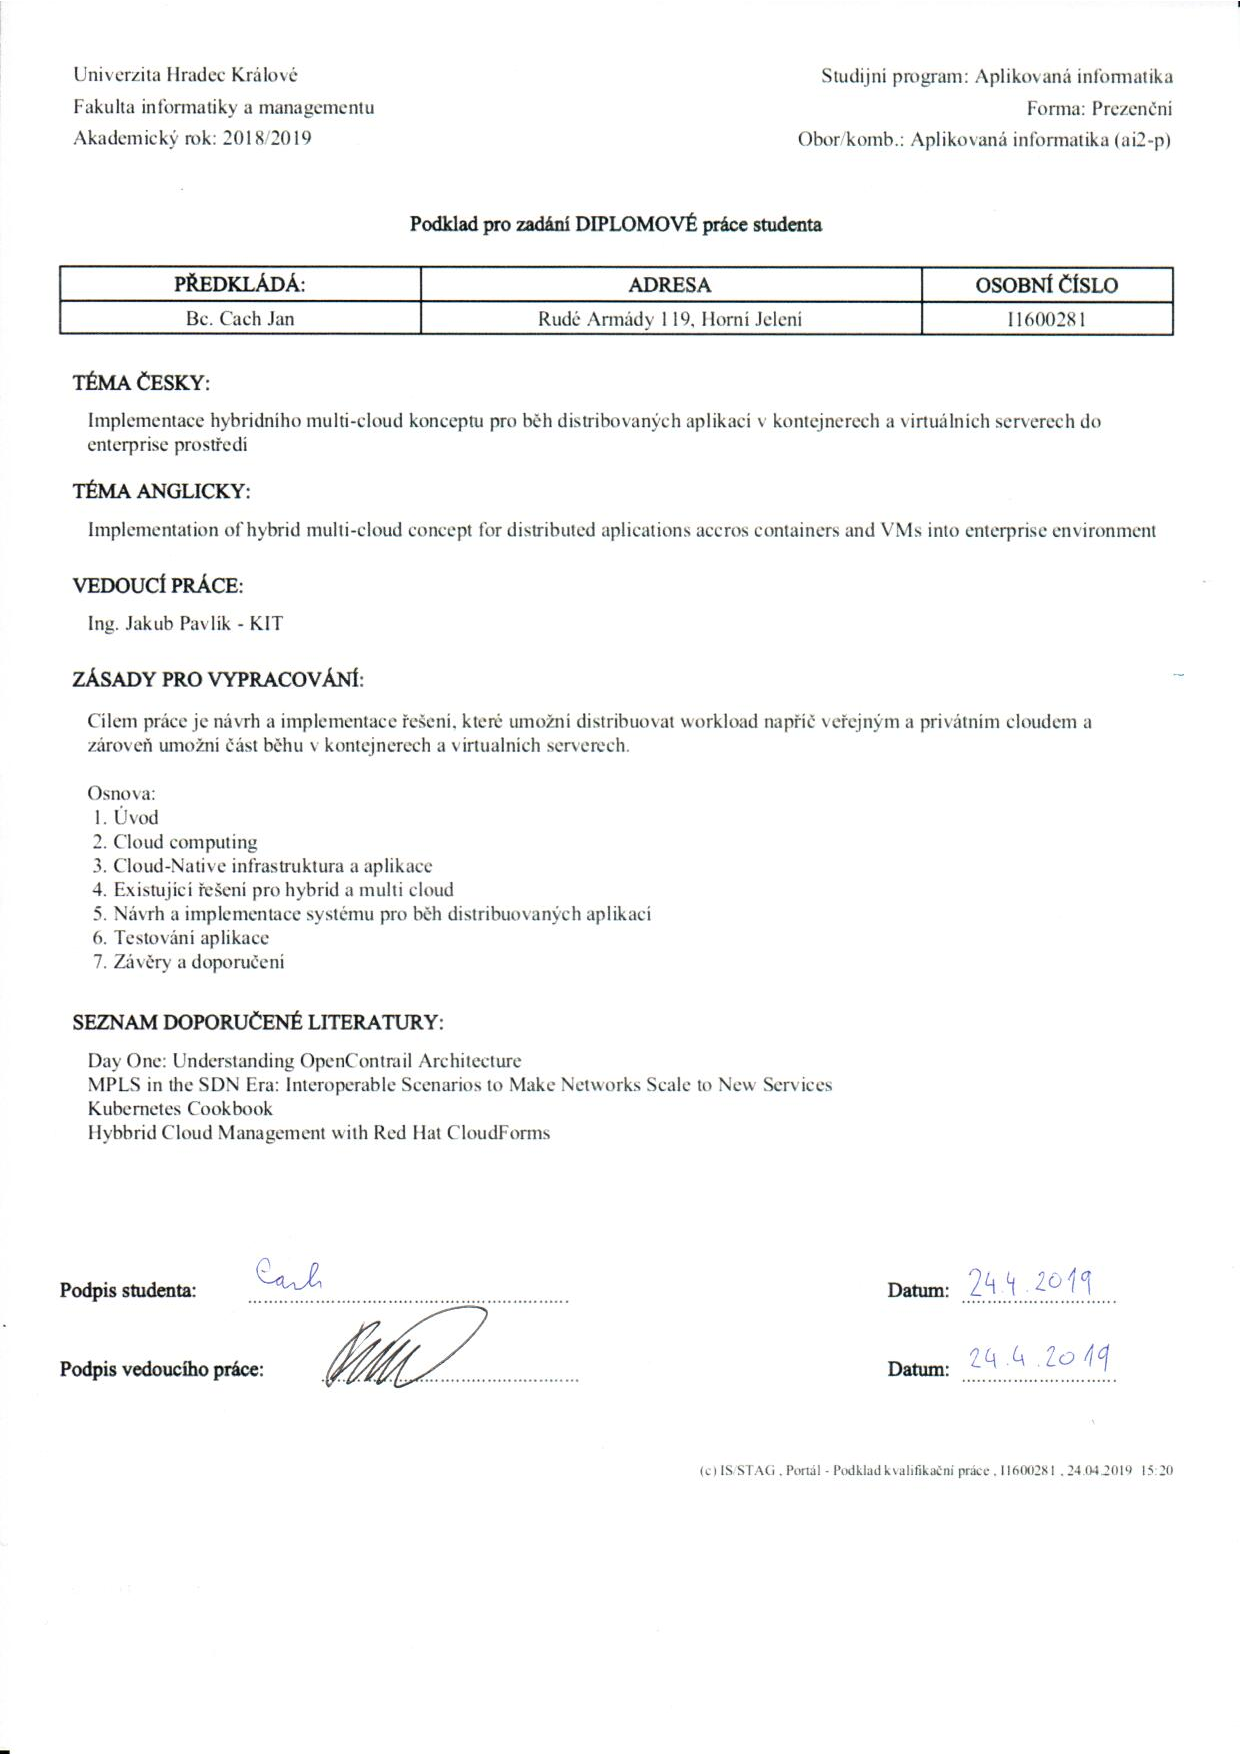
\includepdf[pages={1}]{zadani.pdf}

\clearpage{}
\end{document}
